\documentclass[11pt]{article}
\usepackage{euscript}

\usepackage{amsmath}
\usepackage{amsthm}
\usepackage{amssymb}
\usepackage{epsfig}
\usepackage{xspace}
\usepackage{color}
\usepackage{url}

%%%%%%%%%%%%%%%%%%%%%%%%%%%%%%%%%
\setlength{\textheight}{9in}
\setlength{\topmargin}{-0.600in}
\setlength{\headheight}{0.2in}
\setlength{\headsep}{0.250in}
\setlength{\footskip}{0.5in}
\flushbottom
\setlength{\textwidth}{6.5in}
\setlength{\oddsidemargin}{0in}
\setlength{\evensidemargin}{0in}
\setlength{\columnsep}{2pc}
\setlength{\parindent}{1em}
%%%%%%%%%%%%%%%%%%%%%%%%%%%%%%%%%


\newcommand{\eps}{\varepsilon}

\renewcommand{\c}[1]{\ensuremath{\EuScript{#1}}}
\renewcommand{\b}[1]{\ensuremath{\mathbb{#1}}}
\newcommand{\s}[1]{\textsf{#1}}

\newcommand{\E}{\textbf{\textsf{E}}}
\renewcommand{\Pr}{\textbf{\textsf{Pr}}}

\title{Homework 3 Data Mining
\footnote{\s{CS 6955 Data Mining; \;\; Spring 2012 \hfill
Instructor: Jeff M. Phillips, University of Utah}
}
}
\author{Alex Clemmer}

\begin{document}
\maketitle





%%%%%%%%%%%%%%%%%%%%%%%%%%%%%%%%%%%%%%%%%%%%%%%%%%%%
%%%%%%%%%%%%%%%%%%%%%%%%%%%%%%%%%%%%%%%%%%%%%%%%%%%%
%%%%%%%%%%%%%%%%%%%%%%%%%%%%%%%%%%%%%%%%%%%%%%%%%%%%

\section{Hierarchical Clustering}

\paragraph{A: } 

Mean link probably works the best on large data, since you don't have to compute pairwise norms. It is hard to say which worked ``best", since that depends on your measurement (\textit{i.e.}, inter-cluster similarity, extra-cluster similarity, whether it looks ``good", etc.). That said, it is likely that the min link clustering produced the best-looking results, since the points that should be clustered together tend to be closest to the clusters they should be in.

\textit{Single-Link Clustering:}
\begin{verbatim}
CLUST
('m', (14.02, 5.03))
('n', (16.05, 5.01))
CLUST
('a', (4.01, 15.021))
('b', (3.02, 14.031))
('c', (2.99, 12.02))
('d', (3.107, 10.04))
('e', (3.08, 8.05))
('f', (3.04, 7.03))
('g', (4.01, 6.06))
('h', (5.07, 5.06))
('i', (6.02, 4.03))
('j', (8.06, 4.09))
('k', (10.02, 4.08))
('l', (12.01, 4.07))
CLUST
('o', (12.54, 12.51))
('p', (12.03, 12.04))
('q', (11.52, 11.57))
('r', (11.03, 11.09))
('s', (10.51, 10.532))
('t', (10.01, 10.01))
('u', (12.5, 15.52))
('v', (12.06, 15.1))
('w', (11.55, 14.57))
('x', (11.08, 14.3))
('y', (10.52, 13.53))
('z', (10.03, 13.008))

\end{verbatim}

\textit{Complete-Link Clustering:}
\begin{verbatim}
CLUST
('e', (3.08, 8.05))
('f', (3.04, 7.03))
('g', (4.01, 6.06))
('h', (5.07, 5.06))
('i', (6.02, 4.03))
CLUST
('j', (8.06, 4.09))
('k', (10.02, 4.08))
('l', (12.01, 4.07))
('m', (14.02, 5.03))
('n', (16.05, 5.01))
CLUST
('a', (4.01, 15.021))
('b', (3.02, 14.031))
('c', (2.99, 12.02))
('d', (3.107, 10.04))
('o', (12.54, 12.51))
('p', (12.03, 12.04))
('q', (11.52, 11.57))
('r', (11.03, 11.09))
('s', (10.51, 10.532))
('t', (10.01, 10.01))
('u', (12.5, 15.52))
('v', (12.06, 15.1))
('w', (11.55, 14.57))
('x', (11.08, 14.3))
('y', (10.52, 13.53))
('z', (10.03, 13.008))

\end{verbatim}

\textit{Average-Link Clustering:}
\begin{verbatim}
CLUST
('o', (12.54, 12.51))
('p', (12.03, 12.04))
('q', (11.52, 11.57))
('r', (11.03, 11.09))
('s', (10.51, 10.532))
('t', (10.01, 10.01))
('u', (12.5, 15.52))
('v', (12.06, 15.1))
('w', (11.55, 14.57))
('x', (11.08, 14.3))
('y', (10.52, 13.53))
('z', (10.03, 13.008))
CLUST
('j', (8.06, 4.09))
('k', (10.02, 4.08))
('l', (12.01, 4.07))
('m', (14.02, 5.03))
('n', (16.05, 5.01))
CLUST
('a', (4.01, 15.021))
('b', (3.02, 14.031))
('c', (2.99, 12.02))
('d', (3.107, 10.04))
('e', (3.08, 8.05))
('f', (3.04, 7.03))
('g', (4.01, 6.06))
('h', (5.07, 5.06))
('i', (6.02, 4.03))

\end{verbatim}

\textit{Average-Link Clustering:}
\begin{verbatim}
CLUST
('o', (12.54, 12.51))
('p', (12.03, 12.04))
('q', (11.52, 11.57))
('r', (11.03, 11.09))
('s', (10.51, 10.532))
('t', (10.01, 10.01))
('u', (12.5, 15.52))
('v', (12.06, 15.1))
('w', (11.55, 14.57))
('x', (11.08, 14.3))
('y', (10.52, 13.53))
('z', (10.03, 13.008))
CLUST
('j', (8.06, 4.09))
('k', (10.02, 4.08))
('l', (12.01, 4.07))
('m', (14.02, 5.03))
('n', (16.05, 5.01))
CLUST
('a', (4.01, 15.021))
('b', (3.02, 14.031))
('c', (2.99, 12.02))
('d', (3.107, 10.04))
('e', (3.08, 8.05))
('f', (3.04, 7.03))
('g', (4.01, 6.06))
('h', (5.07, 5.06))
('i', (6.02, 4.03))
\end{verbatim}


\paragraph{B: }

Begin with the definition of the average-link cluster:

\begin{equation}
\cfrac{1}{|S_1||S_2|} \sum_{(s_1,s_2) \in S_1 \times S_2} || s_1 - s_2||_2 = \cfrac{1}{|S_1||S_2|} \sum_{(s_1,s_2) \in S_1 \times S_2} \sqrt{s_1^2 - s_2^2}
\end{equation}

\begin{equation}
= \cfrac{1}{|S_1||S_2|} \sqrt{\sum_{s_1 \in S_1} s_1^2 - \sum_{s_2 \in S_2} s_2^2}
\end{equation}

This is clearly equivalent to the mean cluster, as long as it's $\mathbb{R}^1$.





\section{Point Assignment Clustering}




\section{High Dimensions}

\paragraph{A:} 

I used $n=10,000$ for my histograms. \textbf{First}, the histograms for the $L_1$ norms for increadingly high dimensionality $d$:

\begin{center}
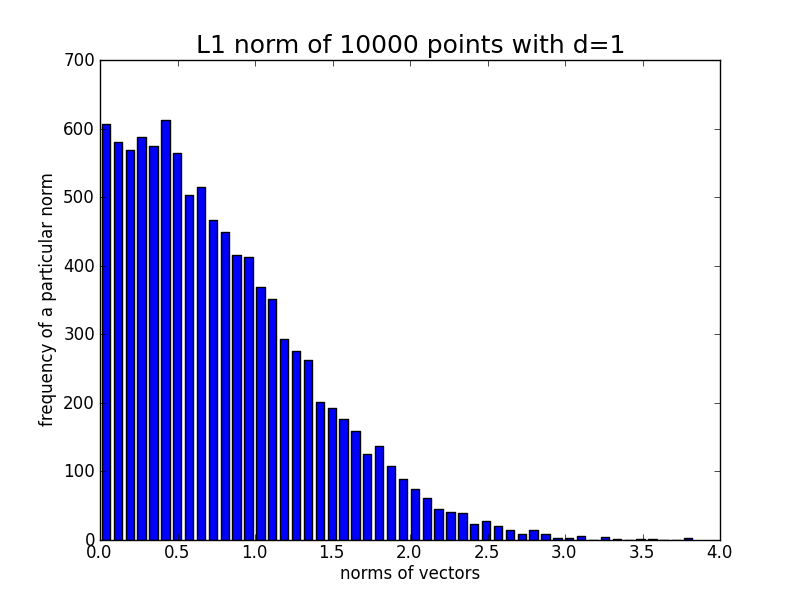
\includegraphics[scale=0.25]{p1d1.png}
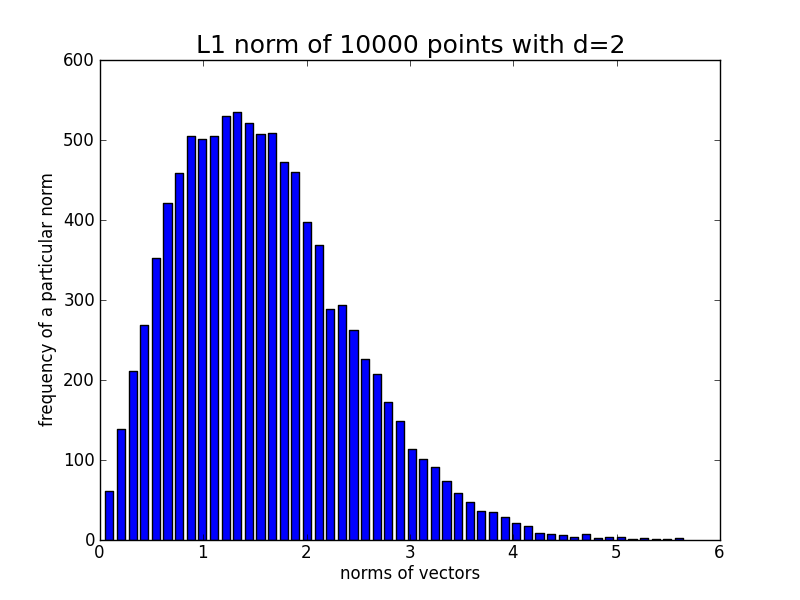
\includegraphics[scale=0.25]{p1d2.png}
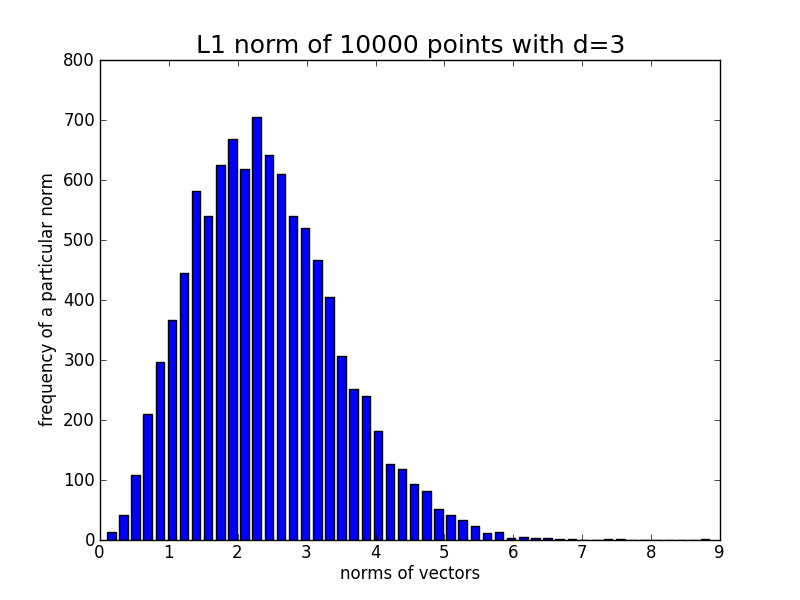
\includegraphics[scale=0.25]{p1d3.png}
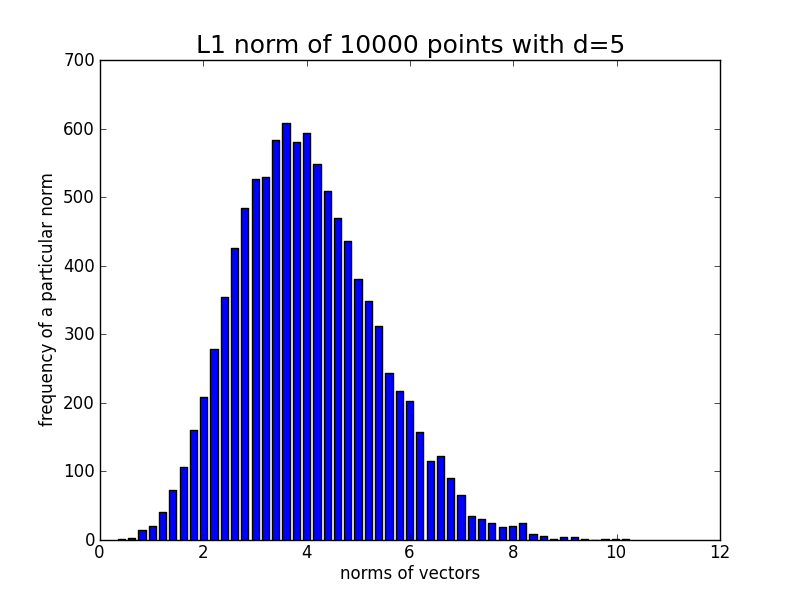
\includegraphics[scale=0.25]{p1d5.png}
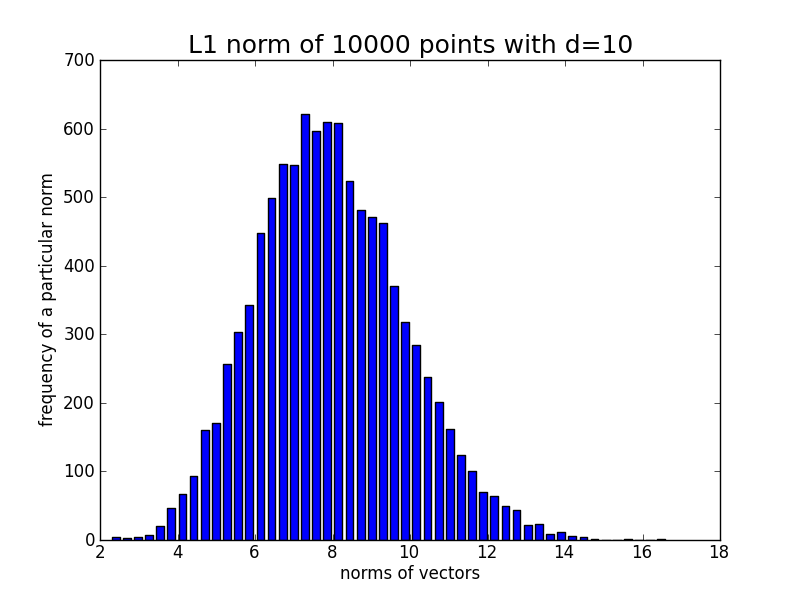
\includegraphics[scale=0.25]{p1d10.png}
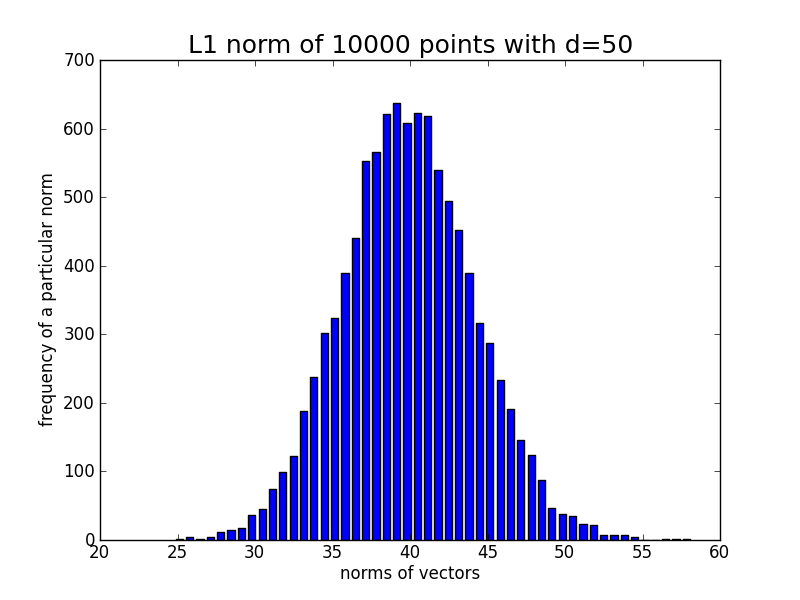
\includegraphics[scale=0.25]{p1d50.png}
\end{center}

And second, the histograms for the $L_2$ norms on increasingly high dimensionality $d$:

\begin{center}
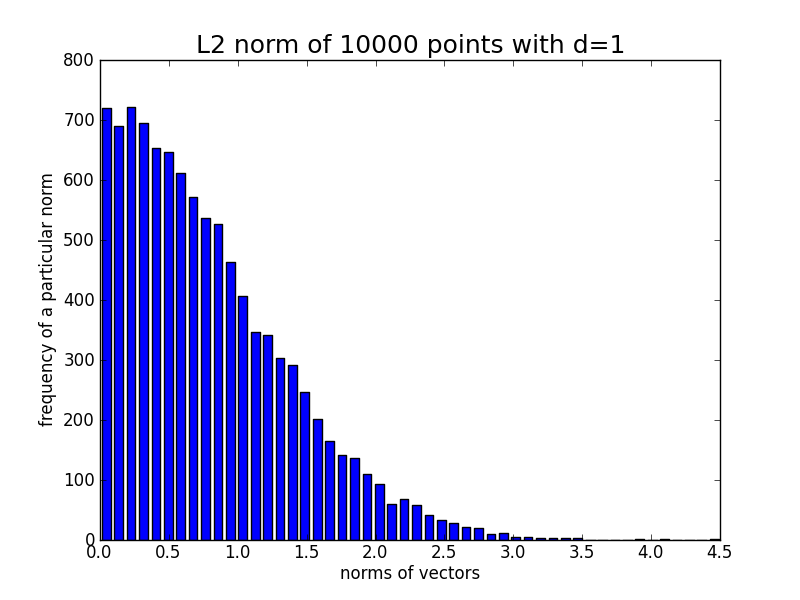
\includegraphics[scale=0.25]{p2d1.png}
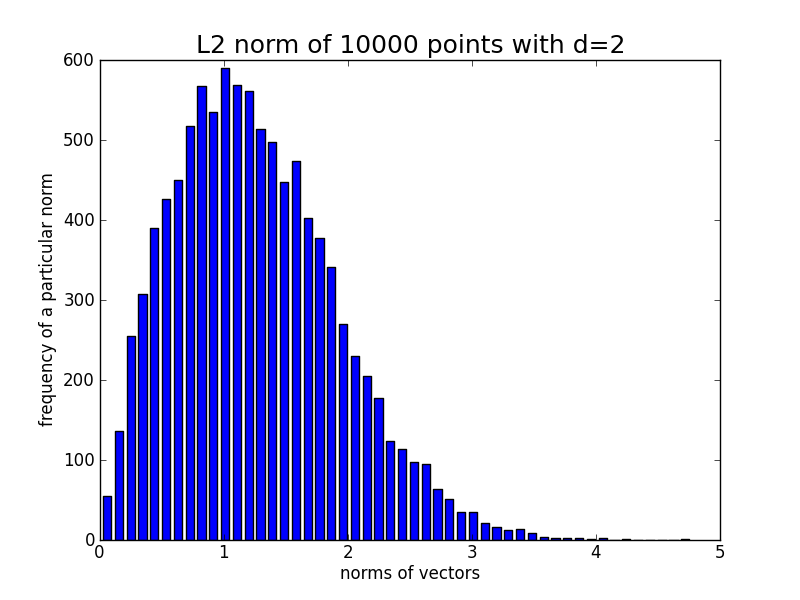
\includegraphics[scale=0.25]{p2d2.png}
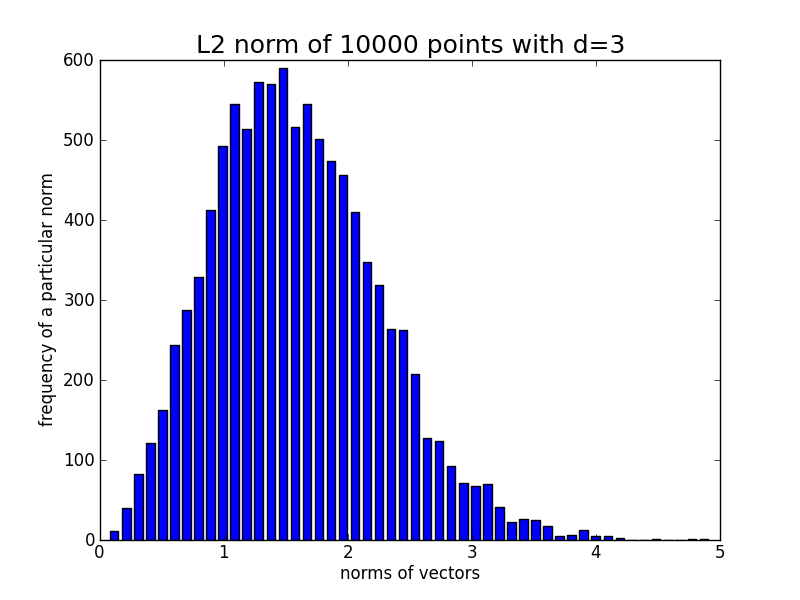
\includegraphics[scale=0.25]{p2d3.png}
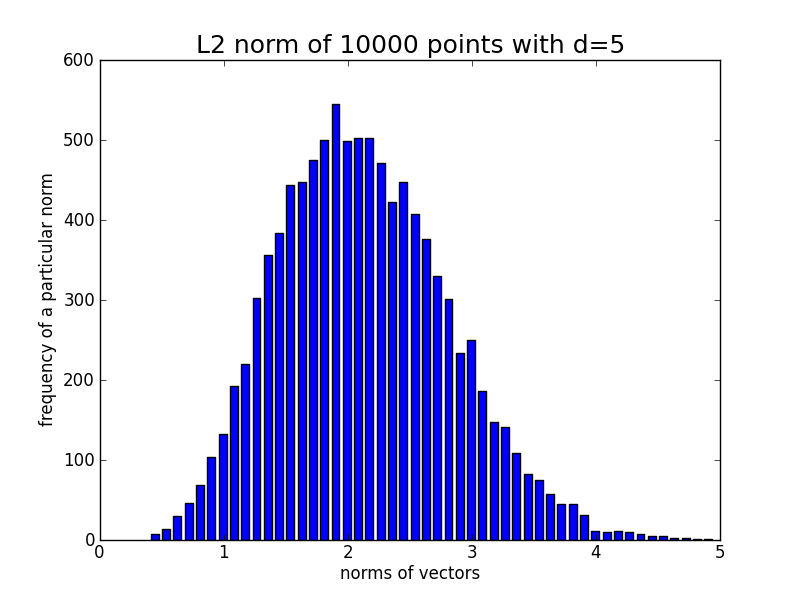
\includegraphics[scale=0.25]{p2d5.png}
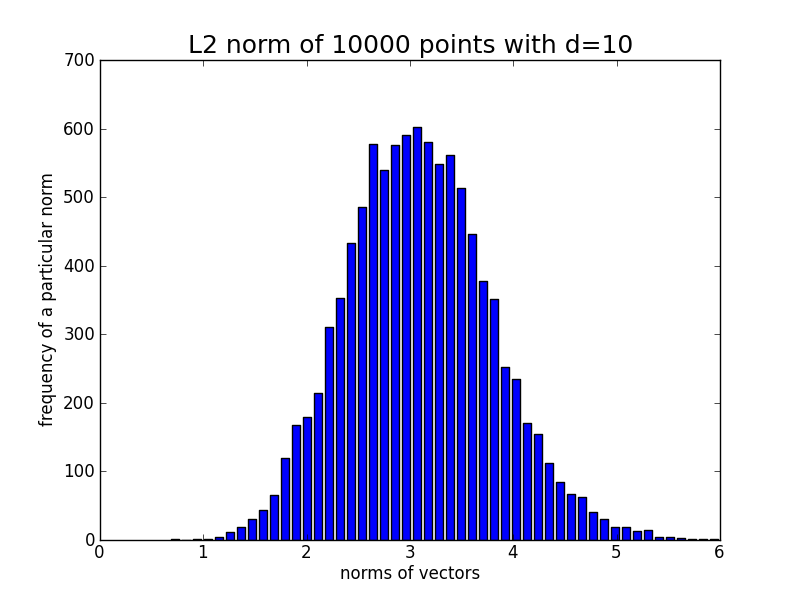
\includegraphics[scale=0.25]{p2d10.png}
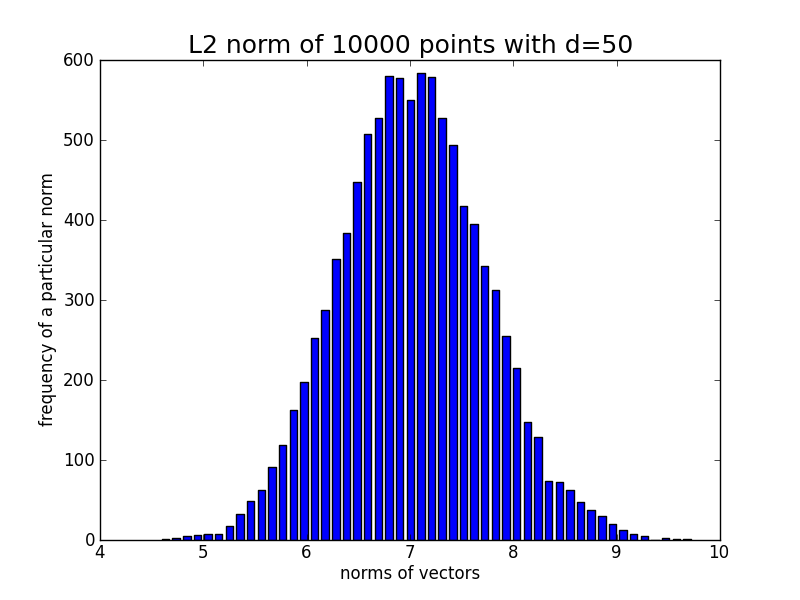
\includegraphics[scale=0.25]{p2d50.png}
\end{center}


\paragraph{B:} 

I estimated the probability by generating $n=10,000$ samples, norming them, and calculating at the empirical $\Pr(L_P(\vec{x})  <1)$ for all $\vec{x}$ in my generated observations.

The tables are broken apart by dimension $d$ (\textit{i.e.}, the first table is for $d=1$, the second for $d = 2$, and so on). The \textit{index} column is just the number of the experiment---it's useful because there should be 30 in all, which we can plainly see. The $P$ column refers to which norm $L_P$ we're using, \textit{e.g.}, $L_1$, $L_2$, and so on.

Finally, (and most importantly) the last column refers to the empirical probability that the norm is less 1. We calculate this by taking the number of samples for which this condition is true, and dividing that number by the total.

\begin{center}
For $d = 1$:

\begin{tabular}{| c || c | c | c |}
\hline
\textit{index} & $d$ & $P$ in $L_P$ & $\Pr(<1)$ \\
\hline
\hline
1 & 1 & 0.5 & 1.000000 \\
\hline
2 & 1 & 1 & 1.000000 \\
\hline
3 & 1 & 2 & 1.000000 \\
\hline
4 & 1 & 3 & 1.000000 \\
\hline
5 & inf & 3.0 & 1.000000 \\
\hline
\end{tabular}

For $d = 2$:

\begin{tabular}{| c || c | c | c |}
\hline
\textit{index} & $d$ & $P$ in $L_P$ & $\Pr(<1)$ \\
\hline
\hline
6 & 2 & 0.5 & 0.166200 \\
\hline
7 & 2 & 1 & 0.501400 \\
\hline
8 & 2 & 2 & 0.785800 \\
\hline
9 & 2 & 3 & 0.883900 \\
\hline
10 & inf & 3.0 & 0.883900 \\
\hline
\end{tabular}

For $d = 3$:

\begin{tabular}{| c || c | c | c |}
\hline
\textit{index} & $d$ & $P$ in $L_P$ & $\Pr(<1)$ \\
\hline
\hline
11 & 3 & 0.5 & 0.011600 \\
\hline
12 & 3 & 1 & 0.158100 \\
\hline
13 & 3 & 2 & 0.523600 \\
\hline
14 & 3 & 3 & 0.706900 \\
\hline
15 & inf & 3.0 & 0.706900 \\
\hline
\end{tabular}

For $d = 5$:

\begin{tabular}{| c || c | c | c |}
\hline
\textit{index} & $d$ & $P$ in $L_P$ & $\Pr(<1)$ \\
\hline
\hline
16 & 5 & 0.5 & 0.000000 \\
\hline
17 & 5 & 1 & 0.008400 \\
\hline
18 & 5 & 2 & 0.160200 \\
\hline
19 & 5 & 3 & 0.369700 \\
\hline
20 & inf & 3.0 & 0.369700 \\
\hline
\end{tabular}

For $d = 10$:

\begin{tabular}{| c || c | c | c |}
\hline
\textit{index} & $d$ & $P$ in $L_P$ & $\Pr(<1)$ \\
\hline
\hline
21 & 10 & 0.5 & 0.000000 \\
\hline
22 & 10 & 1 & 0.000000 \\
\hline
23 & 10 & 2 & 0.002400 \\
\hline
24 & 10 & 3 & 0.035600 \\
\hline
25 & inf & 3.0 & 0.035600 \\
\hline
\end{tabular}

For $d = 50$:

\begin{tabular}{| c || c | c | c |}
\hline
\textit{index} & $d$ & $P$ in $L_P$ & $\Pr(<1)$ \\
\hline
\hline
26 & 50 & 0.5 & 0.000000 \\
\hline
27 & 50 & 1 & 0.000000 \\
\hline
28 & 50 & 2 & 0.000000 \\
\hline
29 & 50 & 3 & 0.000000 \\
\hline
30 & inf & 3.0 & 0.000000 \\
\hline
\end{tabular}
\end{center}









\end{document}
